\section{RSA}

RSA is a widely used public-key cryptosystem. It operates as a block cipher, encrypting a fixed length
amount of data at once. Most RSA used today is 1024 - 4096 bits (which is the length it bits of the 
modulus, and also the approximately the number of bits that can be encrypted per block). 
For this project, we focused on 1024 bit RSA.

An RSA key pair consists of a public key $(n, e)$ and a private key $(n, d)$. $n$ is the modulus,
$e$ is the encryption exponent, and $d$ is the decryption exponent. $n$ is generally a very large number;
the number of bits in $n$ defines the bitsize of the algorithm. For this project, $n$ is a 1024 bit integer,
composed of the product of two primes $p$ and $q$. $e$ and $d$ satisfy the requirement that $e \cdot d = 1 \mod \varphi(n)$,
where $\varphi(n)$ is the Euler Totient function.

Encryption of the plaintext message $m$ is performed by modular exponentiation to produce the ciphertext $c$: $c = m^e \mod n$.
Decryption is performed in the same manner: $m = c^d \mod n$. In order to maintain a 1 to 1 mapping between input messages and output messages,
$m < n$. This sets the block size: if $n$ is a 1024 bit number, then essentially 1023 bits can be encrypted at once.

For this project, we explored accelerating \emph{modular exponentiation}, allowing the encryption and decryption of blocks to be computed on an FPGA.

\subsection{Techniques}
% This section should provide a detailed description of the applications, algorithms, or
% hardware architectures realized in this project. Think critically about the important items to mention
% in order for the reader to understand how your design works without having to look into any code.
% For example, what are the inputs and outputs of the application (or architecture), what are the major
% steps (or modules), and what does each step (or module) achieve? It would be useful to include
% small examples, block diagrams, mathematical formulas, and other visualizations to help explain your
% techniques. Do not include detailed information about your source code as your report should be at a
% high level.

Implementing modular exponentiation required 2 main components: the actual computation, and algorithms to perform
arithmetic on very large numbers.

The fundamental modular exponentiation algorithm is: \footnote{The ``Right-to-left binary method'' from Wikipedia: \url{https://en.wikipedia.org/wiki/Modular_exponentiation}.}

\begin{verbatim}
function modular_pow(base, exponent, modulus)
    if modulus = 1 then return 0
    result := 1
    base := base mod modulus
    while exponent > 0
        if (exponent mod 2 == 1):
           result := (result * base) mod modulus
        exponent := exponent >> 1
        base := (base * base) mod modulus
    return result
\end{verbatim}

This function is trivial to implement, except that it requires performing multiplication and modulus operations on very large numbers.
In particular, since all the numbers involved are 1024 bits, it required performing 2048 bit arithmetic as the intermediate results
could be over 1024 bits.

We represented the 2048 bit numbers 32 digit base $2^{64}$ numbers. \footnote{This representation is based directly off code from possibly-wrong: \url{https://github.com/possibly-wrong/precision/blob/master/math_Unsigned.h}. The code was heavily modified to make it amenable to HLS. \emph{Mathematics and Algorithms for Computer Algebra} by Francis J. Wright was instrumental in making the required modifications (\url{https://people.eecs.berkeley.edu/~fateman/282/F\%20Wright\%20notes/week4.pdf}). The original implementation off all these algorithms comes from Donald Knuth's \emph{Art of Computer Programming, Volume 2: Seminumerical Algorithms}.}
In this notation, a number $a$ is represented as:
$$a = a_{31} \cdot \left ( 2^{64} \right )^{31} + \ldots + a_{2} \cdot \left ( 2^{64} \right )^{2} + a_{1} \cdot \left ( 2^{64} \right )^{1} + a_{0} \cdot \left ( 2^{64} \right )^{0}$$
The coefficients $\left( a_{31}, \ldots, a_2, a_1, a_0 \right )$ are the digits of $a$ in base $2^{64}$, and are stored in an array.

Using this representation, multiplication and division can be performed much in the same way they are performed on paper using ``long multiplication'' and ``long division''. For an in depth explanation of the algorithms involved, see the references above.


\subsection{Implementation}
% This section describe how you implemented your designs. For example, what
% programming languages did you use? Did you take advantage of any third-party libraries? Is your
% implementation purely software, purely hardware, or a mix of both? Which software and/or hardware
% blocks are included in your design, and what hardware device (if any) did you target? In most cases, it
% would be helpful to include block diagrams of your implementation illustrating the flow of data through
% your design, the interconnection between different blocks, and whether each block is implemented
% in software or hardware. As in the previous section, providing meaningful visualizations would help
% the reader better appreciate your work. Please also include one or two interesting aspects of your
% implementation, especially any specific implementation strategies necessary for creating a functionally
% correct design with good performance.
The entire RSA system is implemented in C++, in the "rsa" directory. It uses a mix of both hardware and software, using 
hardware for modular exponentiation, and software for key generation, chunking, and padding. 
For the hardware portion, we targeted the ZedBoard ("xc7z020clg484-1").

Figure \ref{fig:rsaflow} shows the division of work between hardware and software for an encryption flow.
The ``CBC'' software operation refers to Cipher Block Chaining, which is used to turn RSA, which is a block cipher,
into a secure stream cipher. Instead of encrypting each block directly, the XOR of each block with the encrypted previous block
is encrypted. For the first block, the prior block is replaced by a random initialization vector. This ensures that duplicate
blocks in the input do not result in duplicate blocks in the output.

\begin{figure}[h]
\centering
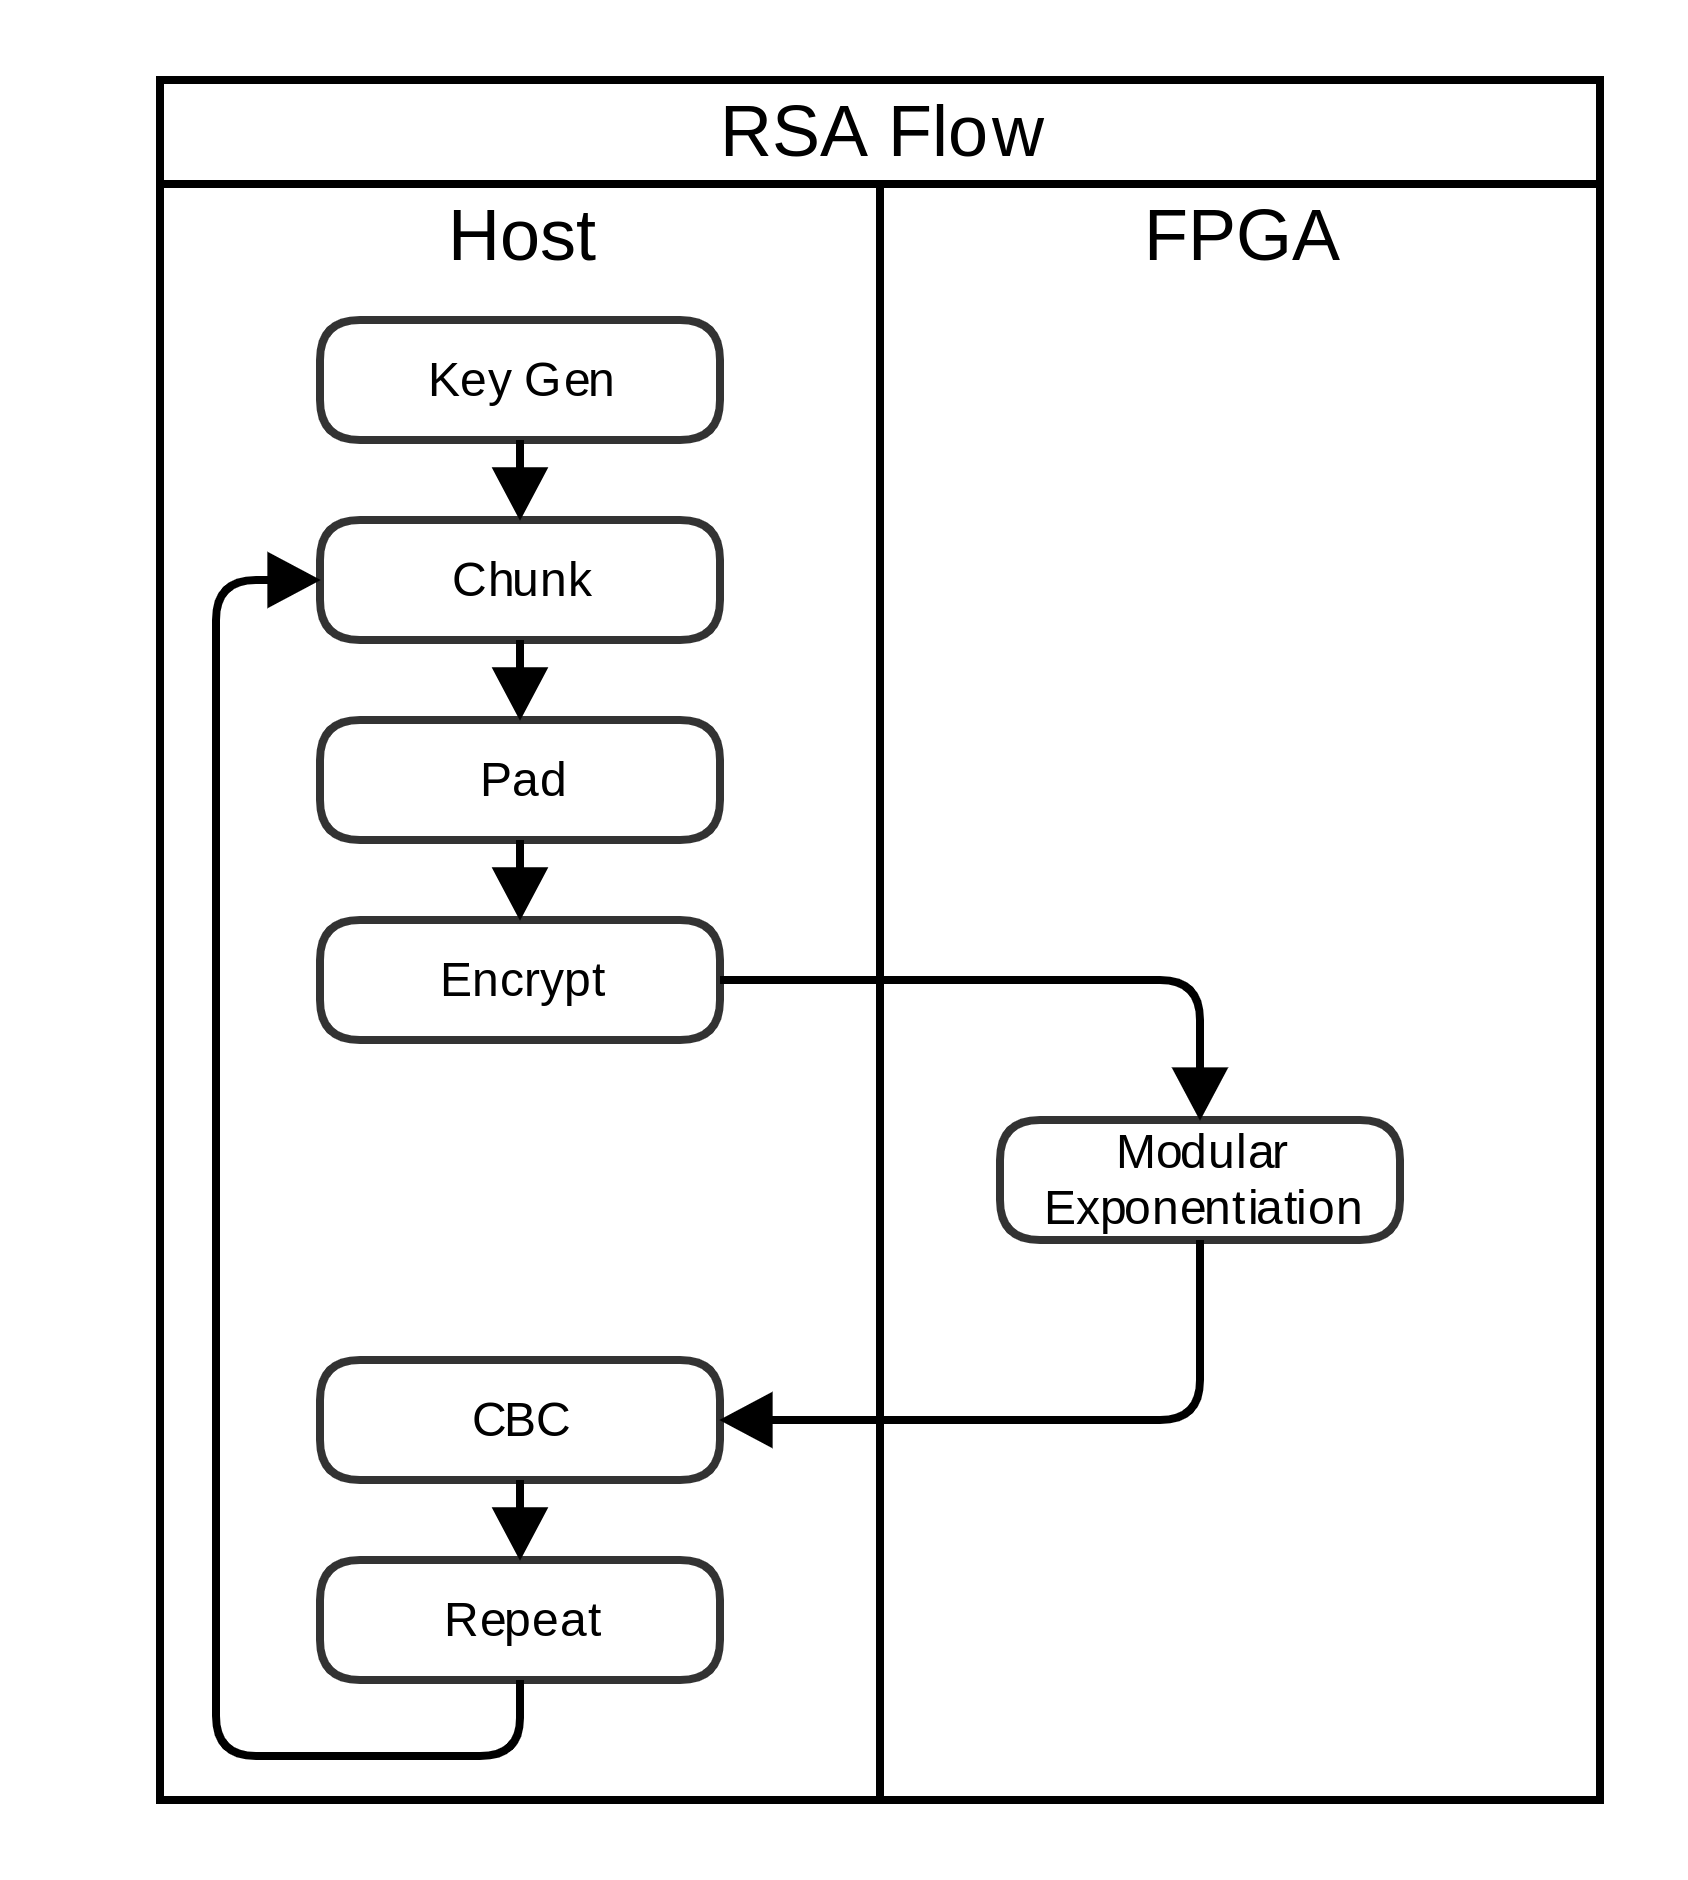
\includegraphics[width=0.5\textwidth]{rsaflow}
\caption{RSA hardware-software system}
\label{fig:rsaflow}
\end{figure}

On the FPGA, the top-level read three 1024 bit numbers (the base $b$, the exponent $e$, and the modulus $n$) from
an input stream, computed $b^e \mod n$, and then wrote the output to a stream.
This top-level module is defined by the "dut" function in "rsa/fpga_rsa.cc".
Communication between the host and FPGA on the ZedBoard is done using the "/dev/xillybus_read_32" and the "/dev/xillybus_write_32"
character devices.

The software portion, "rsa/rsa.cc", takes a message, performs all the key generation, chunking, and padding, and then encrypts
each block using either the FPGA or software.

In addition to the FPGA implementation, we also had 2 software implementations: ``opt'' and ``sim''. The ``opt'' implementation
used the GNU Multiple Precision Arithmetic Library (GMP) to perform modular exponentiation. This library is highly 
optimized. The ``sim'' implementation ran the code to be synthesized directly as C++ code, simulating exactly the computations
carried out on the FPGA.

One unique aspect of our system is that switching between the different implementations of modular exponentiation (either optimal
software, simulated software, or using a real FPGA) can be done with a simple macro definition while compiling "rsa.cc".
When using the provided Makefile ("rsa/Makefile"), the desired mode can be set as follows:
\begin{itemize}
\item Optimal software: "make". Produces the executable "rsa".
\item Simulated software: "make MODE=FPGA_SIM". Produces the executable "rsa-sim".
\item Real FPGA: "make MODE=FPGA_REAL". Produces the executable "rsa-host".
\end{itemize}

\subsection{Evaluation}
% Students should describe the experimental setup used to evaluate their design. Students
% should describe the data inputs used to evaluate their design and provide an analysis of the achieved
% results. The results should be clearly summarized in terms of tables, text, and/or plots. Please provide
% qualitative and quantitative analysis of the results and discuss insights from these results. Results may
% include (but are not limited to) the execution time of an algorithm, hardware resource usage, achievable
% throughput, and error rate. It would be interesting, for example, to discuss why one design is better
% than another, why one design achieves a higher metric than another, or how you trade-off one metric
% for another. Consider going into detail for one particular instance of your experiment and analyze how
% it achieves the given results.

We evaluated both software versions (``opt'' and ``sim'') on both the ZedBoard and ecelinux machines.
The FPGA design was evaluated on the ZedBoard. Due to the complexity of the design, there is not a 
significant baseline design to compare it with. Without the optimization directives, it was difficult
to even get a design that met timing closure. Table \ref{table:rsadata} shows the timing for each implementation
on each computer. The speedup columns (or rather, slowdown) show the speedup relative to the ``fpga-opt'' implementation.
The ``cosim'' row indicates the expected time as given by the HLS co-simulation tool.

Overall, the software implementations are far better than the FPGA implementation. The optimal 
software implementation running on ecelinux (``ecelinux-sw-opt'') was very fast, about 380x faster
than the FPGA implementation for decryption. This is because the GMP library is very well optimized.
Essentially, it is not even using the same algorithms we accelerated, but instead running far more advanced
and complicated algorithms. Even on the ZedBoard, which has a much slower processor than ecelinux, 
the optimized software algorithm is about 30 times faster for encryption than the FPGA.
The simulated software algorithm (which is running the HLS code) is faster, at least for decryption, 
than the ZedBoard CPU.

Overall, however, RSA was really difficult to accelerate. Large number arithmetic has very little obvious parallelism,
and is fraught with dependencies. Furthermore, there is no reason to accelerate it. Since it is known to be slow,
most modern cryptographic algorithms use RSA only to exchange a key for a symmetric algorithm such as AES, and then use AES
for the bulk of the data transfer. PGP is one such algorithm. Given that essentially one RSA block is only used
for a message, and the bulk is another algorithm, it is wasteful to specialize FPGA area for RSA.

\begin{table}[h]
\centering
\begin{tabular}{@{}lllll@{}}
\toprule
Version         & Encrypt (ms) & Decrypt (ms) & Speedup Enc & Speedup Dec \\ \midrule
ecelinux-sw-opt & 0.0355       & 0.627        & 0.00306     & 0.00261     \\
ecelinux-sw-sim & 1.6421       & 112.7        & 0.14161     & 0.46966     \\
zedboard-sw-opt & 0.3997       & 19.478       & 0.03447     & 0.08117     \\
zedboard-sw-sim & 8.1581       & 576.2225     & 0.70353     & 2.40133     \\
fpga-opt        & 11.596       & 239.96       & 1           & 1           \\
cosim           & 3.918        & 234.23       &             &             \\ \bottomrule
\end{tabular}
\label{table:rsadata}
\caption{RSA algorithm runtimes}
\end{table}
